%&template
\documentclass{article}
\usepackage{src/template}

\endofdump
\usepackage{tabularx}
\usepackage{booktabs}


\date{2025 -- 10 -- 26}
\useTemplate[NPA]
\title{NPA -- Cheatsheet}


\begin{document}

    \section{Congestion Control}
    Link Capacity: R\\
    Congestion Window: cwnd 
    Sending Rate: W
    N Hosts
    Ideal throughput: R/N\\
    Measured throughput: \#bytes sent in RTT/RTT\\
    Cost of Congestion(discuss this):
    \begin{itemize}
        \item retransmissions (aka packet got lost send again)
        \item unneeded retransmissions (aka full router buffer \& client sents 2x  )
        \item buffering wasted for packets lost downstream
    \end{itemize}
    Types of Congestion Control:
    \begin{itemize}
        \item loss based: TCP Reno or TCP Cubic
        \item delay based: Vegas (RTT to detect loss)
        \item ECN (explicit markings): L4S
    \end{itemize}
    TCP uses a sliding window to send out packets using the cwnd
    TCP Reno: 3 dupl Ack $\rightarrow$ SR = 1/2\\
    TCP Tahoe: timeout $\rightarrow$  SR = 1 Maximum Segment size\\
    \todo{slow start visualisation}
    TCP slow-start: $2^{cwnd}$ or start with cwnd = 1 and double per round aka cwnd++ for every ack, switch to linear if loss and cwnd is pre loss value \\
    Explicit congestion notification: sender sets ECN bits (01) in IP header, router changes header to 11 if congestion , reciever extracts and sets ECE bit(TCP) on ACK 

    L4S - Low Latency, Low Loss, and Scalable (IPv4 + IPv6):
    \begin{itemize}
        \item no packet drops, marks -> congestion signaling
        \item  no starvation of traffic
        \item marks to control L4S rate
        \item coexists with non-L4S traffic
        \item prioritizes L4S traffic
        \item goals: Max throughput, min latency
        \item Praque theoreme
    \end{itemize}
    Datarate $r = \frac{1}{p}-1[Mbps]$ with packet marking probability $p$ 

    Fairness:
    R/N
    
    UDP sends as constant rate → No Congestion Control
    
    TCP allows multiple parallel connections


    - Wie funktioniert TCP Reno als Visualization

    \section{Packet Classification}

    \subsection{goals}

    \begin{itemize}
        \item Routing Decision $\rightarrow{}$ select interface, fastest Route
        \item Packet filtering $\rightarrow{}$ Drop and Allow traffic
        \item Accounting $\rightarrow{}$ measure the data
        \item rate limiting
    \end{itemize}

    \subsection{binary representation of IPv4}

    %\begin{table}[h]
    %\centering
    %\begin{tabular}{|l|c|c|c|c|}
    %\hline
    %\textbf{IP Address} & 00001100 & 00000100 & 00000000 & 00000000 \\
    %\hline
    %\textbf{Mask} & 11111111 & 11111110 & 00000000 & 00000000 \\
    %\hline
    %\end{tabular}
    %\caption{IP Address 12.4.0.0/15}
    %\end{table}


    \begin{center}
    \textbf{IP Address: 12.4.0.0 \quad IP Mask: 255.254.0.0}
    
    \smallskip
    \begin{tabular}{r|c|c|c|c|}
    \textbf{Address} & \texttt{00001100} & \texttt{00000100} & \texttt{00000000} & \texttt{00000000} \\
    \textbf{Mask}    & \texttt{11111111} & \texttt{11111110} & \texttt{00000000} & \texttt{00000000} \\
    \end{tabular}
    
    \smallskip
    $\xleftarrow{\hspace{1.5cm}}$ \textbf{Network Prefix} $\xrightarrow{\hspace{0.2cm}}$
    $\xleftarrow{\hspace{0.8cm}}$ \textbf{for hosts} $\xrightarrow{\hspace{0.8cm}}$
    
    \smallskip
    \fbox{\textbf{Usually written as 12.4.0.0/15}}
    \end{center}

    \subsection{Unibit Tries}

   \begin{figure}[H]
        \centering
            \begin{tikzpicture}[
                regnode/.style={
                    draw,
                    fill=blue!10,
                    minimum width=4.5cm,
                    minimum height=1.5cm,
                    align=center
                },
                smallreg/.style={
                    draw,
                    fill=blue!10,
                    minimum width=2cm,
                    minimum height=1.5cm,
                    align=center
                },
                bitbox/.style={
                    draw,
                    fill=black,
                    text=white,
                    font=\ttfamily\footnotesize,
                    inner sep=2pt
                }
            ]
    
    
            % #1 Name
            % #2 Position
            % #3 Label
            % #4 Left bit text
            % #5 Right bit text
            \newcommand{\regnodewithbits}[5]{%
                \node[regnode,draw=red] (#1) at #2 {#3};
            
                \node[bitbox, anchor=south west]
                    (#1-bitL) at ($(#1.south west)+(2pt,2pt)$) {#4};
            
                \node[bitbox, anchor=south east]
                    (#1-bitR) at ($(#1.south east)+(-2pt,2pt)$) {#5};
            }
            
            % ---------- Nodes ----------
            \regnodewithbits{R0}{(0,0)}{R0}{00001010}{1100000010101}
            
            \node[smallreg,draw=red] (R1) at (-3,-3) {R1};
            \node[bitbox, anchor=south west]
                (R1-bitL) at ($(R1.south west)+(2pt,2pt)$) {01};
            \node[bitbox, anchor=south east]
                (R1-bitR) at ($(R1.south east)+(-2pt,2pt)$) {1};
            
            \node[smallreg] (R4) at (3,-3) {R4};
            
            \node[smallreg] (R3) at (-4.2,-5) {R3};
            \node[smallreg,draw=red] (R2) at (-1.8,-5) {R2};
            
            % ---------- Edges (now centered under text) ----------
            \draw[->,thick,draw=red] (R0-bitL.south) -- (R1.north);
            \draw[->] (R0-bitR.south) -- (R4.north);
            
            \draw[->] (R1-bitL.south) -- (R3.north);
            \draw[->,thick,draw=red] (R1-bitR.south) -- (R2.north);
            
            \end{tikzpicture}
        \caption{unibit LPM-Trie}
        \end{figure}

        \begin{center}
            Routing Packet P1:
            \begin{align*}
            \text{P1} & ~~~ && 10.128.12.1 &&& = &&&& \textcolor{red}{00001010.1}0000000.00001100.00000001 &&&&& \to\ &&&&&& \text{R2} \\
            \end{align*}
        \end{center}

    \textbf{W-bit prefixes, N prefixes:} \quad $\mathcal{O}(W)$ Lookup \quad $\mathcal{O}(NW)$ Storage \quad $\mathcal{O}(W)$ Updates

    \subsection{Bit Vector}


\subsubsection*{Szenario}

Ein Router besitzt $N = 8$ Regeln. Ein eingehendes Paket soll anhand seiner
5-Tupel-Header-Felder klassifiziert werden:

\medskip
\begin{center}
\textbf{Paket:}
\quad \texttt{<123.25.1.1,\; 124,\; 123.25.4.0,\; 53,\; TCP>}
\end{center}

\medskip
\noindent Die Felder sind: \textit{Source-IP, Source-Port, Dest-IP, Dest-Port, Protokoll}.

\subsubsection*{Regeltabelle}

\begin{center}
\begin{tabular}{lccccc}
\toprule
\textbf{Regel} & \textbf{Source-IP} & \textbf{S-Port} & \textbf{Dest-IP} & \textbf{D-Port} & \textbf{Protokoll} \\
\midrule
Rule 1 & 123.25.1.0/24 & ANY & /0          & 25  & ANY \\
Rule 2 & 123.25.1.0/24 & ANY & /0          & 53  & UDP \\
Rule 3 & 123.25.1.0/24 & ANY & 255.2.3.4/31 & 53 & ANY \\
Rule 4 & 123.25.1.0/24 & ANY & /0          & 23  & ANY \\
Rule 5 & 123.25.2.0/24 & 123 & 123.25.3.0/24 & 123 & UDP \\
Rule 6 & /0            & ANY & 123.25.0.0/16 & ANY & ANY \\
Rule 7 & 123.25.0.0/16 & ANY & /0          & ANY & TCP \\
Rule 8 & /0            & ANY & /0          & ANY & ANY \\
\bottomrule
\end{tabular}
\end{center}

\subsubsection*{Bit-Vektoren pro Feld}

F\"{u}r jedes Header-Feld wird gepr\"{u}ft, welche Regeln auf den Paketwert
passen. Das Ergebnis ist ein Bit-Vektor der L\"{a}nge~8.

\medskip
\begin{center}
\begin{tabular}{lccccccccl}
\toprule
\textbf{Feld} & \textbf{R1} & \textbf{R2} & \textbf{R3} & \textbf{R4} &
\textbf{R5} & \textbf{R6} & \textbf{R7} & \textbf{R8} & \textbf{Paketwert} \\
\midrule
Source-IP  & 1 & 1 & 1 & 1 & 0 & 1 & 1 & 1 & 123.25.1.1 \\
Source-Port & 1 & 1 & 1 & 1 & 0 & 1 & 1 & 1 & 124 \\
Dest-IP    & 1 & 1 & 0 & 1 & 0 & 1 & 1 & 1 & 123.25.4.0 \\
Dest-Port  & 0 & 1 & 1 & 0 & 0 & 1 & 1 & 1 & 53 \\
Protokoll  & 1 & 0 & 1 & 1 & 0 & 1 & 1 & 1 & TCP \\
\midrule
\textbf{AND} & \textbf{0} & \textbf{0} & \textbf{0} & \textbf{0} &
\textbf{0} & \textbf{1} & \textbf{1} & \textbf{1} & \\
\bottomrule
\end{tabular}
\end{center}

\subsubsection*{Ergebnis}

Der AND-Vektor ergibt:

\[
B_{\text{AND}} = (0,\, 0,\, 0,\, 0,\, 0,\, 1,\, 1,\, 1)
\]

Es gibt drei Treffer: Rule~6, Rule~7 und Rule~8. Bei der Linear Search wird
das \textbf{erste (h\"{o}chstpriore) Bit} von links gew\"{a}hlt:

\medskip
\begin{center}
$\Rightarrow$ \textbf{Rule 6} wird angewendet
\quad (Source /0, Dest 123.25.0.0/16, ANY, ANY)
\end{center}

\subsubsection*{Komplexit\"{a}t}

\begin{center}
\begin{tabular}{ll}
\toprule
Zeitkomplexit\"{a}t & $O(N \cdot d)$ \quad ($N$ = Regeln, $d$ = Felder) \\
Speicher            & $O(N \cdot d)$ Bits \\
\bottomrule
\end{tabular}
\end{center}

\noindent Mit Bitparallelit\"{a}t (Wortbreite $W$) reduziert sich der AND-Schritt
auf $O(N/W)$ pro Feld.



    %%% 

    \section{Subnets}
    From our Homework:
    
    \begin{tikzpicture}
        \node (image) at (0,0) {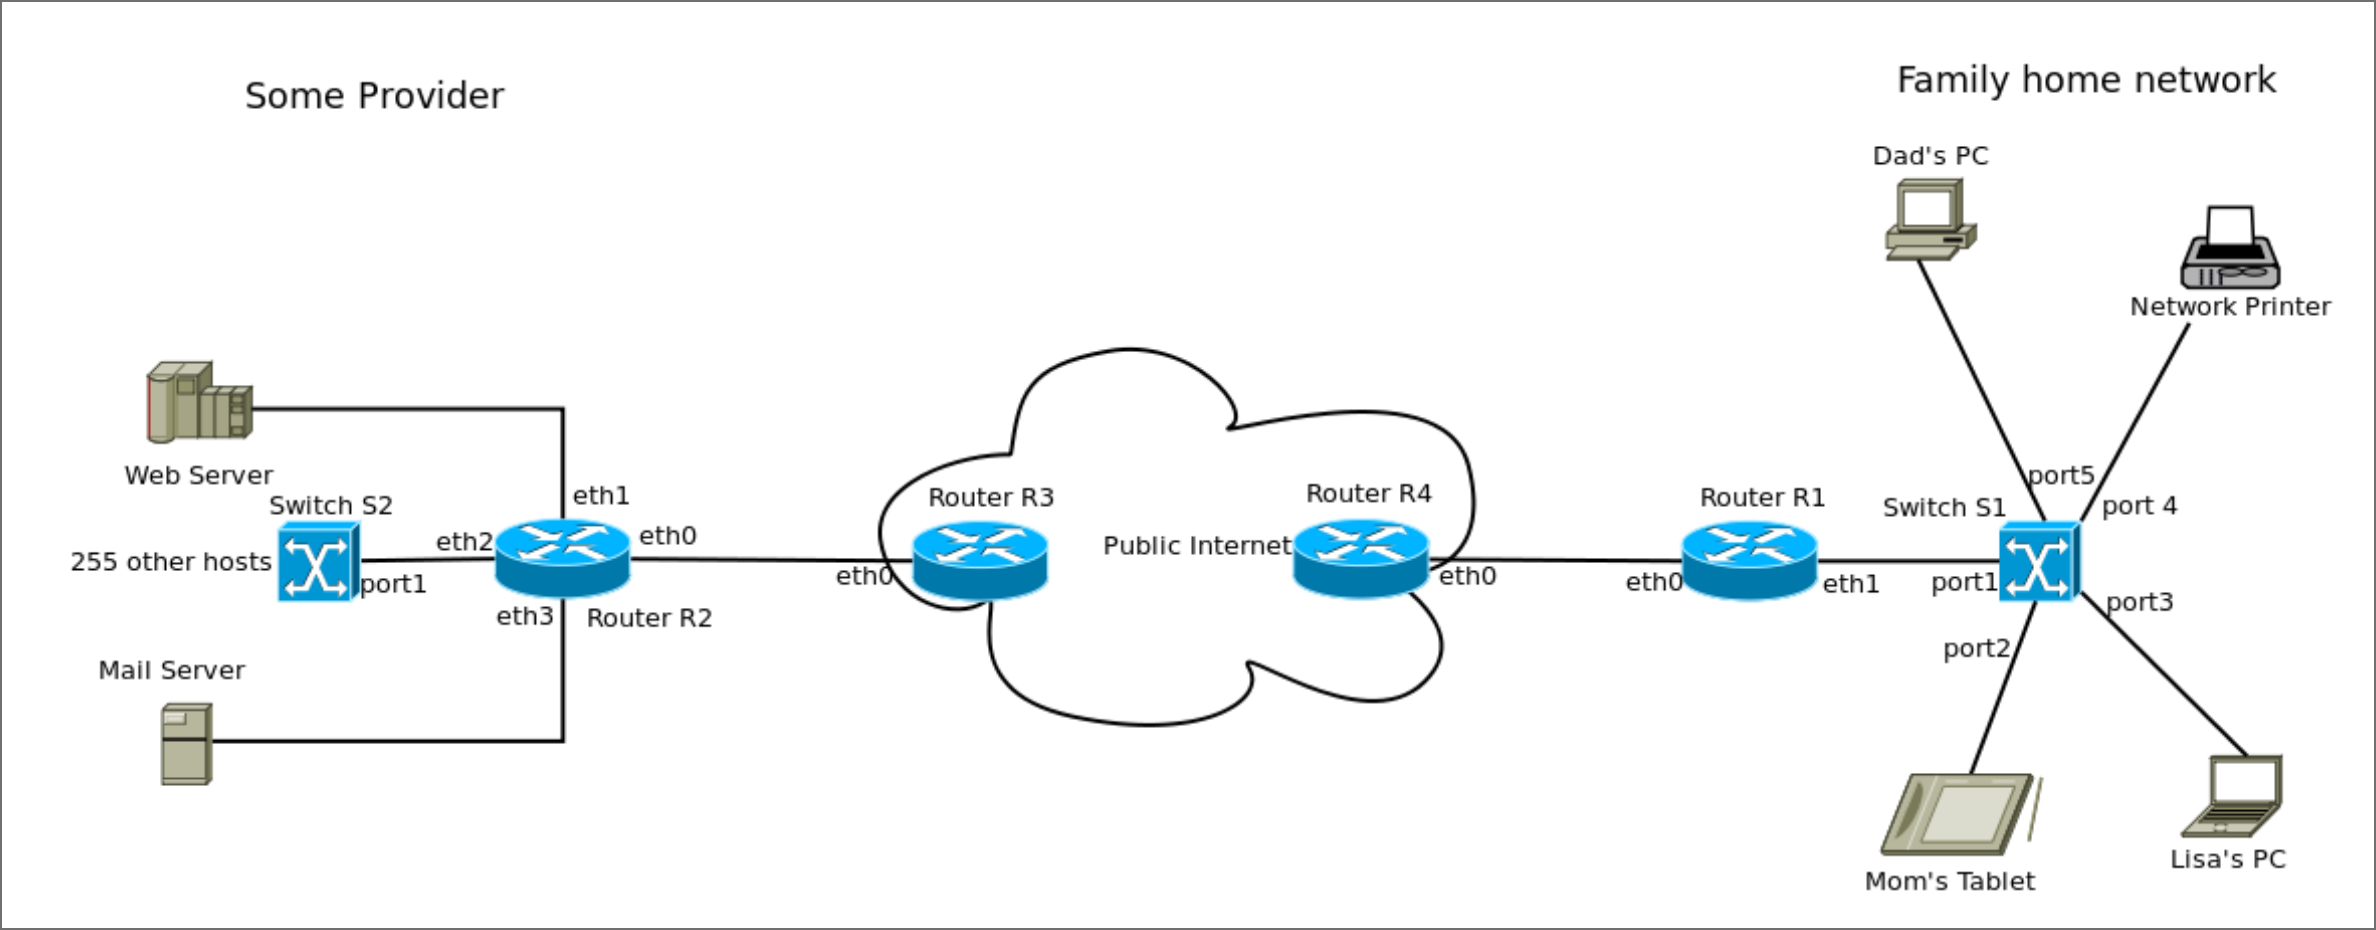
\includegraphics[width=\textwidth]{images/Ex 5a.png}};
        \draw[Orchid, ultra thick] (6.25,0) ellipse (2.1cm and 4.2cm);
        \draw[ForestGreen, ultra thick] (-6.45,-0.7) ellipse (1.7cm and 0.52cm);
        \draw[Orange, ultra thick] (-4.7, -0.4) -- (-4.7, -0.18) -- (-8, -0.18) -- (-8, 1) -- (-4, 1) -- (-4, -0.66);
        \draw[LightSeaGreen, ultra thick] (-4.95, -0.8) -- (-4.95, -1.35) -- (-8, -1.35) -- (-8, -2.5) -- (-4, -2.5) -- (-4, -0.66);

        \draw[blue, ultra thick] (2.7, -0.66) ellipse (1.2cm and 0.5cm);
        \draw[red, ultra thick] (-3, -0.66) ellipse (1.2cm and 0.5cm);
    \end{tikzpicture}



\end{document}